\chapter{Wyniki i wnioski}  
\label{cha:wyniki}  

W tym rozdziale przedstawiono wyniki i wnioski z eksperymentów przeprowadzonych dla algorytmów \textit{L*}, \textit{RPNI}, \textit{GIG} oraz \textit{ALERGIA}. Celem eksperymentów była analiza skuteczności, wydajności oraz zdolności do uogólniania danych przez każdą z metod. Tabele i wykresy ilustrują zależności między parametrami wejściowymi a metrykami, takimi jak liczba stanów w automatach, liczba zapytań oraz czas wykonania. Każdy algorytm testowano na odpowiednio dobranych danych, aby uwzględnić jego specyficzne właściwości i ograniczenia.


\section{Algorytm \textit{L*}}  
W tej sekcji przedstawiono wyniki eksperymentów przeprowadzonych dla algorytmu \textit{L*}. Analizowano liczbę zapytań oraz rozmiar wynikowego automatu w zależności od złożoności problemu. 

Tabele \ref{tab:lstar_prefix} oraz \ref{tab:lstar_blocks} przedstawiają wyniki eksperymentów. Kolumna \textit{Rozmiar problemu (\(n\))} określa poziom złożoności testowanego języka. Kolumny \textit{EQ} oraz \textit{MQ} zawierają odpowiednio liczbę zapytań o równoważność hipotez oraz przynależność, które były wymagane do skonstruowania poprawnego modelu. Ostatnia kolumna, \textit{Rozmiar DFA}, wskazuje liczbę stanów w wynikowym automacie deterministycznym (\textit{DFA}).

Jak pokazano na wykresie \ref{fig:lstar_prefix_mq}, liczba zapytań o przynależność (\textit{MQ}) rośnie wykładniczo wraz ze wzrostem rozmiaru problemu (\(n\)). Liczba zapytań o równoważność (\textit{EQ}) pozostaje natomiast niewielka, co sugeruje, że algorytm efektywnie formułuje hipotezy dotyczące struktury języka. Rozmiar wynikowego automatu (\textit{DFA}) rośnie liniowo w stosunku do złożoności problemu, co potwierdza zdolność algorytmu do uogólniania danych przy zachowaniu minimalnej liczby stanów. Wyniki pokrywają się z liczbą stanów minimalnego automatu, opisaną wzorem \( n + 2 \).

Wyniki przedstawione na wykresie \ref{fig:lstar_blocks_mq} również wskazują wykładniczy wzrost liczby zapytań (\textit{MQ}) wraz z rozmiarem problemu. W tym przypadku odnotowano większą liczbę zapytań o równoważność (\textit{EQ}) w porównaniu do poprzedniego eksperymentu, co sugeruje, że algorytm wymaga więcej prób do rozpoznania bardziej złożonych wzorców. Liczba zapytań o równoważność zależy od specyfiki problemu i może być trudna do przewidzenia. Rozmiar automatu (\textit{DFA}) rośnie liniowo, co potwierdza minimalność modelu, zgodnie ze wzorem \( 2n + 2 \).

\begin{table}[ht]
\centering
\caption{Wyniki eksperymentu z sekcji \ref{sec:eksperyment1}.}
\label{tab:lstar_prefix}
\begin{tabular}{|c|c|c|c|}
\hline
Rozmiar problemu (\(n\)) & EQ & MQ & Rozmiar DFA \\ \hline
1                        & 2  & 13 & 3           \\ \hline
2                        & 3  & 25 & 4           \\ \hline
4                        & 3  & 61 & 6           \\ \hline
8                        & 3  & 181 & 10         \\ \hline
16                       & 3  & 613 & 18         \\ \hline
32                       & 3  & 2245 & 34        \\ \hline
64                       & 3  & 8581 & 66        \\ \hline
\end{tabular}
\end{table}

\begin{figure}[ht]
\centering
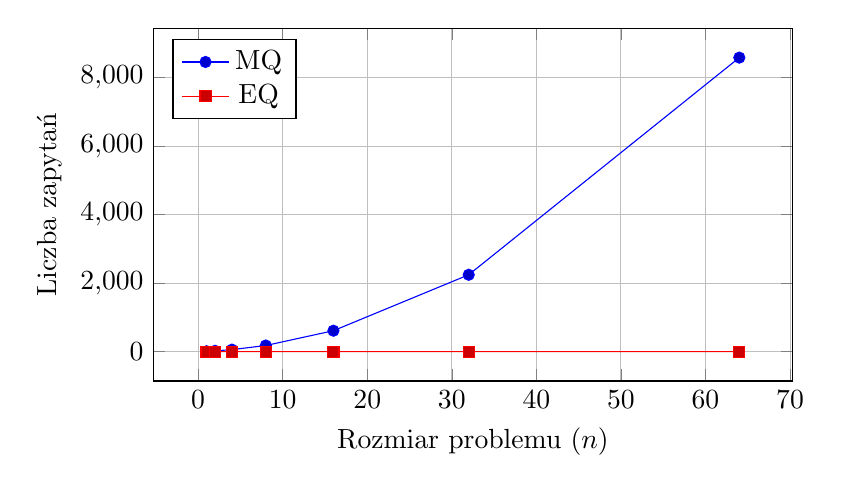
\begin{tikzpicture}
\begin{axis}[
    xlabel={Rozmiar problemu (\(n\))},
    ylabel={Liczba zapytań},
    legend pos=north west,
    grid=major,
    width=0.8\textwidth,
    height=0.5\textwidth
]

% MQ
\addplot coordinates {(1, 13) (2, 25) (4, 61) (8, 181) (16, 613) (32, 2245) (64, 8581)};
\addlegendentry{MQ}

% EQ
\addplot coordinates {(1, 2) (2, 3) (4, 3) (8, 3) (16, 3) (32, 3) (64, 3)};
\addlegendentry{EQ}

\end{axis}
\end{tikzpicture}
\caption{Zależność liczby zapytań EQ i MQ od rozmiaru problemu dla języka z sekcji \ref{sec:eksperyment1}.}
\label{fig:lstar_prefix_mq}
\end{figure}

\begin{table}[ht]
\centering
\caption{Wyniki eksperymentu z sekcji \ref{sec:eksperyment2}.}
\label{tab:lstar_blocks}
\begin{tabular}{|c|c|c|c|}
\hline
Rozmiar problemu (\(n\)) & EQ & MQ & Rozmiar DFA \\ \hline
1                        & 3  & 24  & 4           \\ \hline
2                        & 4  & 54  & 6           \\ \hline
3                        & 5  & 104 & 8           \\ \hline
4                        & 6  & 180 & 10          \\ \hline
5                        & 7  & 288 & 12          \\ \hline
6                        & 8  & 434 & 14          \\ \hline
7                        & 9  & 624 & 16          \\ \hline
8                        & 10 & 864 & 18          \\ \hline
9                        & 11 & 1160 & 20         \\ \hline
\end{tabular}
\end{table}

\begin{figure}[ht]
\centering
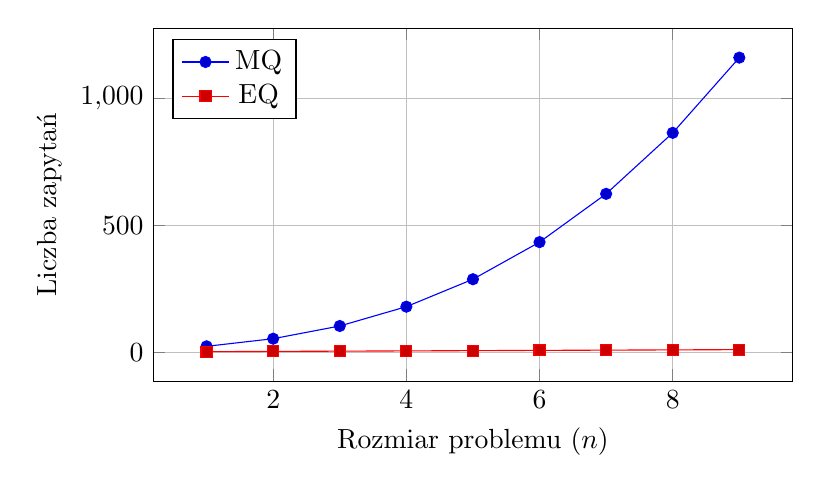
\begin{tikzpicture}
\begin{axis}[
    xlabel={Rozmiar problemu (\(n\))},
    ylabel={Liczba zapytań},
    legend pos=north west,
    grid=major,
    width=0.8\textwidth,
    height=0.5\textwidth
]

% MQ
\addplot coordinates {(1, 24) (2, 54) (3, 104) (4, 180) (5, 288) (6, 434) (7, 624) (8, 864) (9, 1160)};
\addlegendentry{MQ}

% EQ
\addplot coordinates {(1, 3) (2, 4) (3, 5) (4, 6) (5, 7) (6, 8) (7, 9) (8, 10) (9, 11)};
\addlegendentry{EQ}

\end{axis}
\end{tikzpicture}
\caption{Zależność liczby zapytań EQ i MQ od rozmiaru problemu dla języka z sekcji \ref{sec:eksperyment2}.}
\label{fig:lstar_blocks_mq}
\end{figure}


\section{Algorytm \textit{RPNI}}  
Eksperymenty dla algorytmu \textit{RPNI} miały na celu ocenę wpływu rozmiaru alfabetu na czas działania oraz strukturę wynikowego automatu. Testy przeprowadzono na językach z ciągami rozpoczynającymi się symbolem \( 0 \), po którym mogły występować dowolne symbole z danego alfabetu. Dane testowe przygotowano tak, aby liczba stanów w drzewie prefiksów (\textit{PTA}) była zbliżona dla różnych konfiguracji, co zapewniło porównywalność wyników.  

Tabela \ref{tab:rpni_results} przedstawia szczegóły wyników eksperymentu. Kolumna \textit{Rozmiar alfabetu (\(|\Sigma|\))} określa liczbę symboli w alfabecie testowego języka, a \textit{Liczba przykładów} podaje łączną liczbę danych wejściowych. Kolumny \textit{Stany PTA} i \textit{Stany DFA} przedstawiają odpowiednio liczbę stanów w drzewie prefiksów i wynikowym automacie deterministycznym (\textit{DFA}). Ostatnia kolumna, \textit{Czas [s]}, zawiera czas wykonania algorytmu.  

Wyniki pokazują, że czas działania algorytmu rośnie wraz z rozmiarem alfabetu (rys. \ref{fig:rpni_time}), choć dla alfabetu o rozmiarze 64 odnotowano krótszy czas niż dla 32. Może to wynikać ze specyfiki danych testowych lub procesu łączenia stanów. Liczba stanów w wynikowym automacie pozostaje niska, co świadczy o skuteczności algorytmu w uogólnianiu danych, jednak dla większych alfabetów (\(|\Sigma| = 16\) i \(|\Sigma| = 32\)) obserwuje się niewielki wzrost liczby stanów, co może sugerować trudności w uogólnianiu przypadków ze średnim rozmiarem alfabetu.  

Porównywalna liczba stanów w \textit{PTA} dla różnych rozmiarów alfabetów zapewniła rzetelność wyników, eliminując wpływ różnic w danych wejściowych. Algorytm \textit{RPNI} zachowuje wydajność przy różnych konfiguracjach parametrów, choć czas działania rośnie dla większych alfabetów.

\begin{table}[ht]
\centering
\caption{Wyniki dla algorytmu \textit{RPNI}.}
\label{tab:rpni_results}
\begin{tabular}{|c|c|c|c|c|}
\hline
Rozmiar alfabetu (\(|\Sigma|\)) & Liczba przykładów & Stany PTA & Stany DFA & Czas [s] \\ \hline
\num{2}                         & \num{2807}        & \num{5508.44} & \num{3.00}      & \num{0.105} \\ \hline
\num{4}                         & \num{1821}        & \num{4993.48} & \num{3.00}      & \num{0.166} \\ \hline
\num{8}                         & \num{1673}        & \num{5675.68} & \num{3.00}      & \num{0.364} \\ \hline
\num{16}                        & \num{1673}        & \num{5307.78} & \num{3.58}   & \num{0.644} \\ \hline
\num{32}                        & \num{2257}        & \num{5103.64} & \num{4.50}   & \num{1.080} \\ \hline
\num{64}                        & \num{4561}        & \num{4756.92} & \num{3.06}   & \num{0.883} \\ \hline
\end{tabular}
\end{table}

\begin{figure}[ht]
\centering
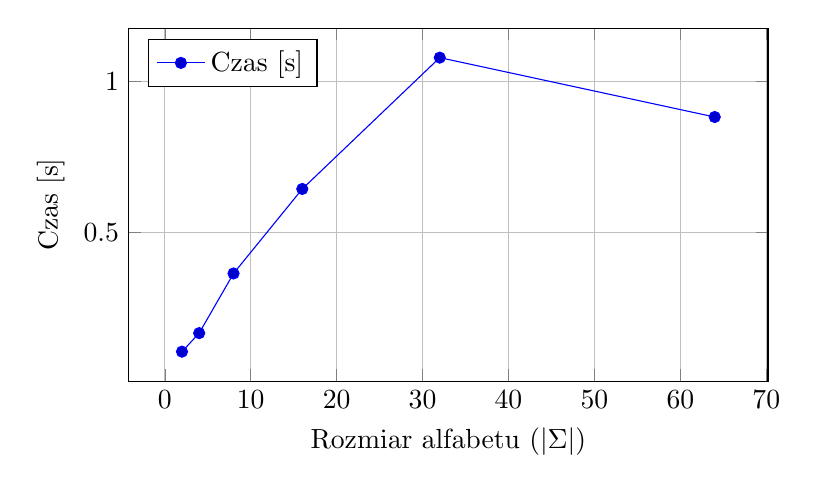
\begin{tikzpicture}
\begin{axis}[
    xlabel={Rozmiar alfabetu (\(|\Sigma|\))},
    ylabel={Czas [s]},
    legend pos=north west,
    grid=major,
    width=0.8\textwidth,
    height=0.5\textwidth
]
\addplot coordinates {(2, 0.104656) (4, 0.166168) (8, 0.364098) (16, 0.644382) (32, 1.08004) (64, 0.883063)};
\addlegendentry{Czas [s]}
\end{axis}
\end{tikzpicture}
\caption{Zależność czasu wykonania algorytmu RPNI od rozmiaru alfabetu.}
\label{fig:rpni_time}
\end{figure}


\section{Algorytm \textit{GIG}}  
Przeprowadzone eksperymenty dla algorytmu \textit{GIG} miały na celu zbadanie wpływu metody inicjalizacji populacji na jakość wynikowego automatu, liczbę generacji potrzebnych do uzyskania rozwiązania oraz dokładność klasyfikacji danych testowych.

Tabele \ref{tab:gig_one_a}, \ref{tab:gig_even_a} oraz \ref{tab:gig_even_a_or_b} prezentują wyniki uzyskane dla różnych metod inicjalizacji populacji. Kolumna \emph{Inicjalizacja populacji} określa zastosowany sposób inicjalizacji -- \emph{warstwowa} oznacza podejście opisane w sekcji \ref{sec:gig-formalizacja}, natomiast \emph{losowa} generuje populację bez dodatkowych założeń. Kolumna \emph{Pokolenie} przedstawia średnią liczbę pokoleń potrzebnych do znalezienia rozwiązania. Kolumna \emph{Jakość} podaje skuteczność modelu jako procent poprawnych klasyfikacji. Kolumny \emph{TP} (\textit{True Positives}) i \emph{TN} (\textit{True Negatives}) wskazują odsetek poprawnych klasyfikacji przykładów pozytywnych i negatywnych, natomiast kolumny \emph{FP} (\textit{False Positives}) i \emph{FN} (\textit{False Negatives}) pokazują odsetek błędnych klasyfikacji.

Obie metody inicjalizacji populacji osiągnęły wysoką jakość klasyfikacji w każdym teście, lecz metoda losowa przyniosła lepsze rezultaty, skracając czas konwergencji średnio o $5.42$ pokolenia w teście trzecim (tabela \ref{tab:gig_even_a_or_b}). Sugeruje to, że losowość skuteczniej eksploruje przestrzeń rozwiązań, zwiększając prawdopodobieństwo znalezienia optymalnych modeli. 

Analiza wyników pokazuje, że metoda losowej inicjalizacji była bardziej efektywna dla złożonych języków, podczas gdy dla prostszych obie metody osiągały podobne rezultaty. Różnice w liczbie generacji okazały się niewielkie, co wskazuje, że wybór metody inicjalizacji miał większy wpływ na jakość wynikowych modeli niż na tempo konwergencji algorytmu.


\begin{table}[ht]
\centering
\caption{Wyniki dla języka „Co najmniej jedno \( a \)” z sekcji \ref{sec:eksperyment4}.}
\label{tab:gig_one_a}
\begin{tabular}{|l|c|c|c|c|c|c|}
\hline
Inicjalizacja populacji & Pokolenie & Jakość & TP & TN & FP & FN \\ \hline
Inicjalizacja warstwowa & \num{94.64} & \num{0.944} & \num{0.889} & \num{1} & \num{0.111} & \num{0} \\ \hline
Inicjalizacja losowa    & \num{91.46} & \num{0.943} & \num{0.887} & \num{1} & \num{0.113} & \num{0} \\ \hline
\end{tabular}
\end{table}

\begin{table}[ht]
\centering
\caption{Wyniki dla języka „Parzysta liczba \( a \)” z sekcji \ref{sec:eksperyment5}.}
\label{tab:gig_even_a}
\begin{tabular}{|l|c|c|c|c|c|c|}
\hline
Inicjalizacja populacji & Pokolenie & Jakość & TP & TN & FP & FN \\ \hline
Inicjalizacja warstwowa & \num{95.7}  & \num{0.974} & \num{1} & \num{0.945} & \num{0} & \num{0.055} \\ \hline
Inicjalizacja losowa    & \num{96.44} & \num{0.987} & \num{1} & \num{0.973} & \num{0} & \num{0.028} \\ \hline
\end{tabular}
\end{table}

\begin{table}[ht]
\centering
\caption{Wyniki dla języka „Parzysta liczba \( a \) lub \( b \)” z sekcji \ref{sec:eksperyment6}.}
\label{tab:gig_even_a_or_b}
\begin{tabular}{|l|c|c|c|c|c|c|}
\hline
Inicjalizacja populacji & Pokolenie & Jakość & TP & TN & FP & FN \\ \hline
Inicjalizacja warstwowa & \num{96.2}  & \num{0.923} & \num{0.97}  & \num{0.875} & \num{0.03}  & \num{0.125} \\ \hline
Inicjalizacja losowa    & \num{90.78} & \num{0.968} & \num{0.988} & \num{0.948} & \num{0.013} & \num{0.053} \\ \hline
\end{tabular}
\end{table}


\section{Algorytm \textit{ALERGIA}}  
Badania nad algorytmem \textit{ALERGIA} skupiały się na ocenie jego odporności na szum w danych wejściowych. Analizowano jakość wynikowego modelu oraz liczbę stanów w wynikowym automacie w zależności od poziomu zakłóceń.

Podsumowanie wyników eksperymentu przedstawiono w tabeli \ref{tab:alergia_results}. Kolumna \textit{Procent szumu} określa poziom zakłóceń w danych wejściowych. Kolumna \textit{Jakość} podaje dokładność modelu jako odsetek poprawnych klasyfikacji wśród 10000 słów wygenerowanych z wynikowego automatu. Kolumna \textit{Stany automatu} wskazuje liczbę stanów w wynikowym automacie, co pozwala ocenić złożoność struktury modelu. Wszystkie wartości są uśrednione na podstawie powtórzeń testu.

Jak pokazują tabela \ref{tab:alergia_results} oraz wykresy \ref{fig:alergia_quality} i \ref{fig:alergia_states}, jakość modelu spada wraz ze wzrostem poziomu szumu w danych. Dla niskich zakłóceń (do 2\%) algorytm utrzymuje jakość powyżej 89\%, jednak przy 50\% szumu dokładność spada do około 74\%.  

Liczba stanów w wynikowym automacie wzrasta wraz z poziomem zakłóceń, co wskazuje na trudności w uogólnianiu danych przy większym szumie. Przy zakłóceniach do 10\% liczba stanów pozostaje stabilna, natomiast przy wyższych wartościach rośnie zauważalnie, odzwierciedlając większą złożoność modelu.

Wyniki eksperymentów pokazują, że algorytm \textit{ALERGIA} dobrze radzi sobie z niewielkimi zakłóceniami, zachowując wysoką jakość klasyfikacji i kompaktową strukturę automatu. W miarę wzrostu poziomu szumu jego zdolność do poprawnego odwzorowania języka stopniowo maleje, co objawia się zarówno spadkiem dokładności, jak i wzrostem liczby stanów automatu.

\begin{table}[ht]
\centering
\caption{Wyniki dla algorytmu \textit{ALERGIA}.}
\label{tab:alergia_results}
\begin{tabular}{|c|c|c|}
\hline
Procent szumu & Jakość & Stany automatu \\ \hline
\num{0.000}  & \num{1.000} & \num{2.00}         \\ \hline
\num{0.001}  & \num{0.994} & \num{2.00}         \\ \hline
\num{0.005}  & \num{0.973} & \num{2.14}         \\ \hline
\num{0.010}  & \num{0.953} & \num{2.56}         \\ \hline
\num{0.020}  & \num{0.928} & \num{3.30}         \\ \hline
\num{0.050}  & \num{0.892} & \num{3.92}         \\ \hline
\num{0.100}  & \num{0.898} & \num{4.00}         \\ \hline
\num{0.200}  & \num{0.910} & \num{4.00}         \\ \hline
\num{0.300}  & \num{0.866} & \num{4.32}         \\ \hline
\num{0.400}  & \num{0.799} & \num{4.98}         \\ \hline
\num{0.500}  & \num{0.741} & \num{5.36}         \\ \hline
\end{tabular}
\end{table}

\begin{figure}[ht]
\centering
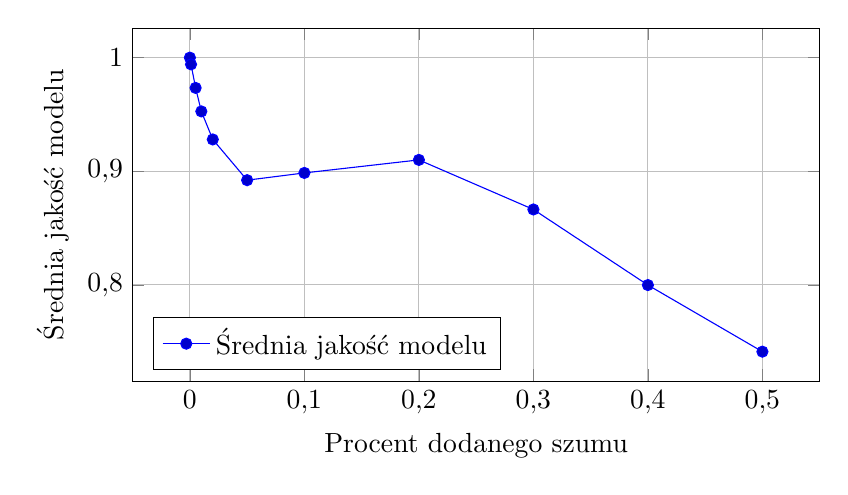
\begin{tikzpicture}
\begin{axis}[
    xlabel={Procent dodanego szumu},
    ylabel={Średnia jakość modelu},
    legend pos=south west,
    grid=major,
    width=0.85\textwidth,
    height=0.5\textwidth,
    x tick label style={/pgf/number format/use comma, /pgf/number format/1000 sep={\,}},
    y tick label style={/pgf/number format/use comma, /pgf/number format/1000 sep={\,}}
]
\addplot coordinates {(0, 1.0) (0.001, 0.994074) (0.005, 0.97336) (0.01, 0.95268) (0.02, 0.927988) (0.05, 0.892144) (0.1, 0.898522) (0.2, 0.909984) (0.3, 0.866366) (0.4, 0.799828) (0.5, 0.741206)};
\addlegendentry{Średnia jakość modelu}
\end{axis}
\end{tikzpicture}
\caption{Zależność jakości modelu od poziomu szumu w danych.}
\label{fig:alergia_quality}
\end{figure}

\begin{figure}[ht]
\centering
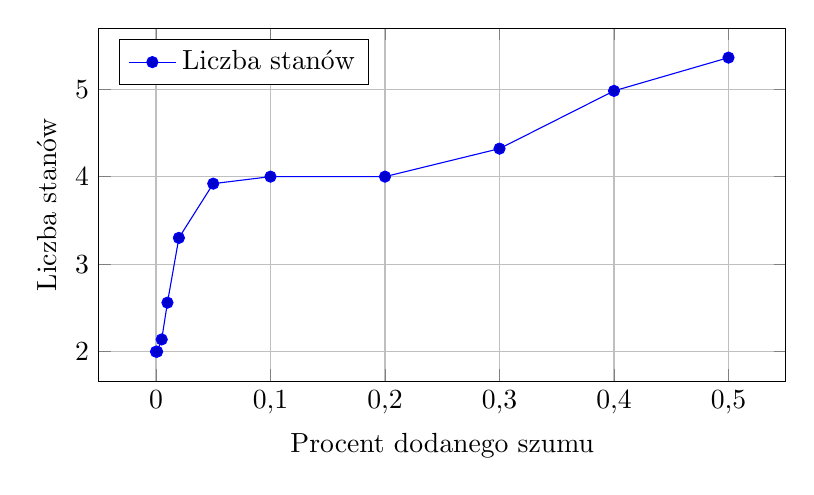
\begin{tikzpicture}
\begin{axis}[
    xlabel={Procent dodanego szumu},
    ylabel={Liczba stanów},
    legend pos=north west,
    grid=major,
    width=0.85\textwidth,
    height=0.5\textwidth,
    x tick label style={/pgf/number format/use comma, /pgf/number format/1000 sep={\,}},
    y tick label style={/pgf/number format/use comma, /pgf/number format/1000 sep={\,}}
]
\addplot coordinates {(0, 2) (0.001, 2) (0.005, 2.14) (0.01, 2.56) (0.02, 3.3) (0.05, 3.92) (0.1, 4) (0.2, 4) (0.3, 4.32) (0.4, 4.98) (0.5, 5.36)};
\addlegendentry{Liczba stanów}
\end{axis}
\end{tikzpicture}
\caption{Zależność liczby stanów wynikowego automatu od poziomu szumu dodanego do danych.}
\label{fig:alergia_states}
\end{figure}


\section{Podsumowanie}  
Przeprowadzone eksperymenty pozwoliły na ocenę skuteczności i wydajności algorytmów \textit{L*}, \textit{RPNI}, \textit{GIG} oraz \textit{ALERGIA}. Algorytm \textit{L*} efektywnie generował minimalne automaty deterministyczne (\textit{DFA}), utrzymując niską liczbę zapytań o równoważność (\textit{EQ}), choć liczba zapytań o przynależność (\textit{MQ}) rosła wykładniczo wraz ze złożonością problemu, co czyni go odpowiednim w sytuacjach z dobrze zdefiniowanymi źródłami wiedzy. Algorytm \textit{RPNI} wyróżniał się prostotą, niską złożonością i wysoką wydajnością, co czyni go dobrym wyborem do szybkiego uogólniania danych, niezależnie od rozmiaru alfabetu. Algorytm \textit{GIG}, oparty na metodach ewolucyjnych, oferował elastyczność, lecz jego większa złożoność i czasochłonność nie zawsze przekładały się na lepsze wyniki w porównaniu z prostszymi metodami, a eksperymenty wykazały, że losowa inicjalizacja populacji częściej prowadziła do lepszych wyników niż inicjalizacja warstwowa. Algorytm \textit{ALERGIA} okazał się odporny na niewielkie zakłócenia, zachowując wysoką jakość klasyfikacji i kompaktową strukturę modelu, jednak jego skuteczność spadała przy większym poziomie szumu, co czyni go bardziej odpowiednim do danych probabilistycznych o umiarkowanym poziomie zakłóceń.  

Wybór algorytmu powinien być zatem dostosowany do specyfiki problemu -- \textit{L*} sprawdza się tam, gdzie dostępna jest wyrocznia wysokiej jakości, \textit{RPNI} oferuje szybkość i prostotę, \textit{GIG} nadaje się do złożonych problemów optymalizacyjnych, a \textit{ALERGIA} jest przydatna w modelowaniu danych probabilistycznych.  

Możliwości dalszego rozwoju obejmują powtórzenie eksperymentów na bardziej złożonych lub rzeczywistych danych, co pozwoliłoby na dokładniejsze zbadanie praktycznych zastosowań algorytmów. Ponadto warto przeprowadzić dodatkowe analizy dla innych metod indukcji gramatyk formalnych, które nie zostały uwzględnione w tej pracy, w celu poszerzenia porównania i oceny ich skuteczności w różnych warunkach.
